\section{Testing}
\subsection{Analisi statica}
Per l'analisi statica del codice è stato utilizzato il tool STAN4J, integrato nel IDE Eclipse.
Inserire report?
\todo{Ho visto che un gruppo lo ha inserito alla fine di tutto.}

\subsection{Analisi dinamica}
Nell'iterazione 2 si sono testate tutte le API Rest implementate, utlizzando Postman (\Fig \ref{fig:RisultatiTestAPIIT2}). In particolare si sono testate le seguenti funzionalità:

\begin{itemize}
	\item UserController:
	\begin{itemize}
		\item Login con credenziali corrette e verifica che le informazioni dell'utente ricevute siano corrette;
		\item Login con credenziali errate;
		\item Visualizzazione di tutti gli utenti registrati nel sistema;
		\item Visualizzazione di un utente specifico e verifica corretta dei dati ritornati;
		\item Eliminazione utente;
		\item Inserimento di un nuovo utente e verifica che i dati dell'utente siano stati inseriti in modo corretto;
		\item Modifica utente e verifica che l'utente sia stato modificato correttamente;
	\end{itemize}
	\item TeamController:
	\begin{itemize}
		\item Visualizzazione di una squadra e verifica che le informazioni ricevute siano corrette;
		\item Visualizzazione di tutte le squadre inserite nel sistema;
		\item Eliminazione di una squadra;
		\item Inserimento di una nuova squadra;
	\end{itemize}
	\item AreaController:
	\begin{itemize}
		\item Visualizzazione di tutte le aree inserite nel sistema;
	\end{itemize}

	\begin{figure}[h!]
		\centering
		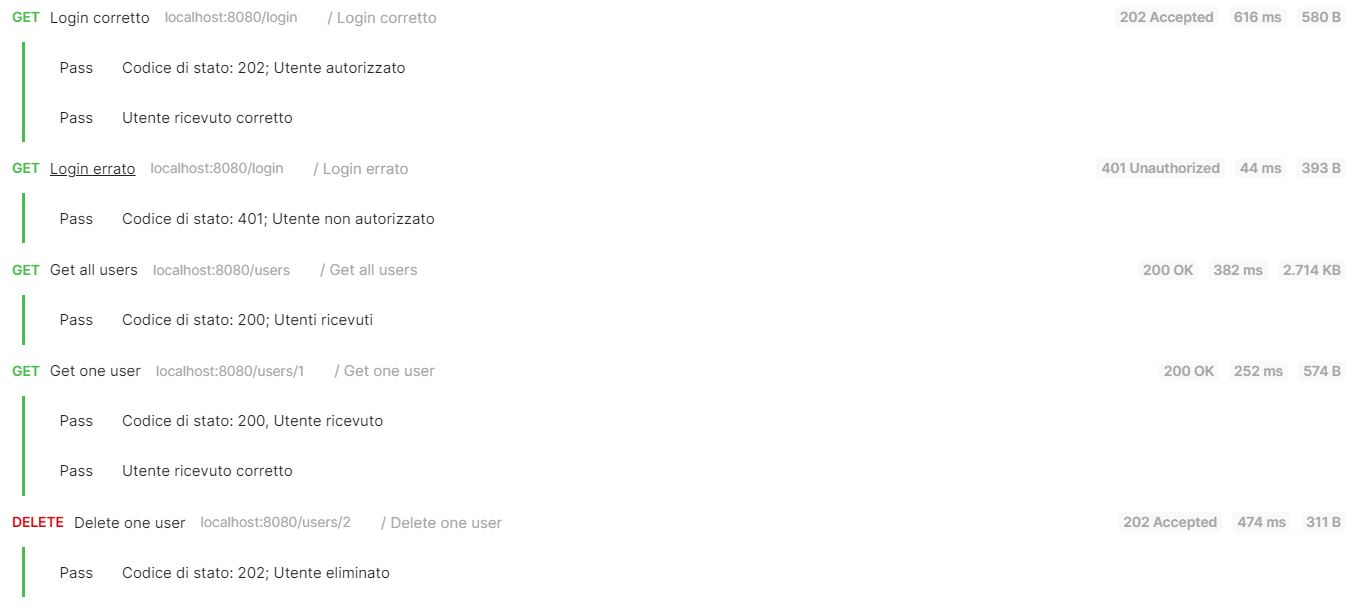
\includegraphics[width=0.99\linewidth]{./Iterazione 2/ImageFiles/TestUserController1}
		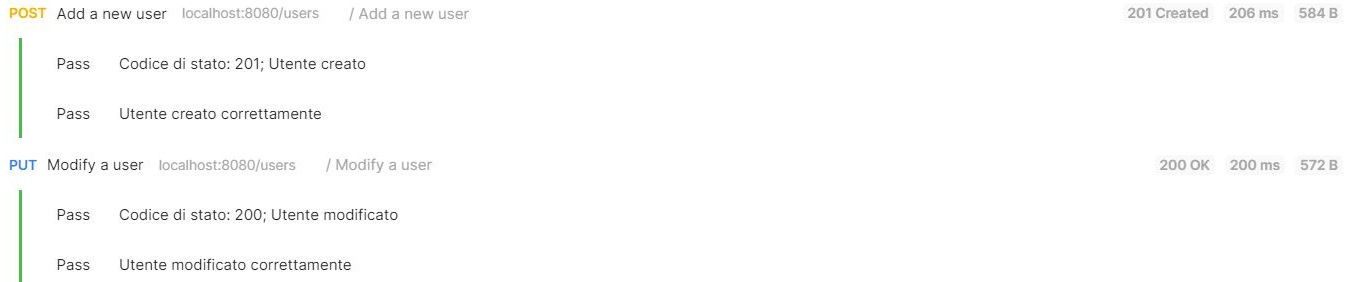
\includegraphics[width=0.99\linewidth]{./Iterazione 2/ImageFiles/TestUserController2}
		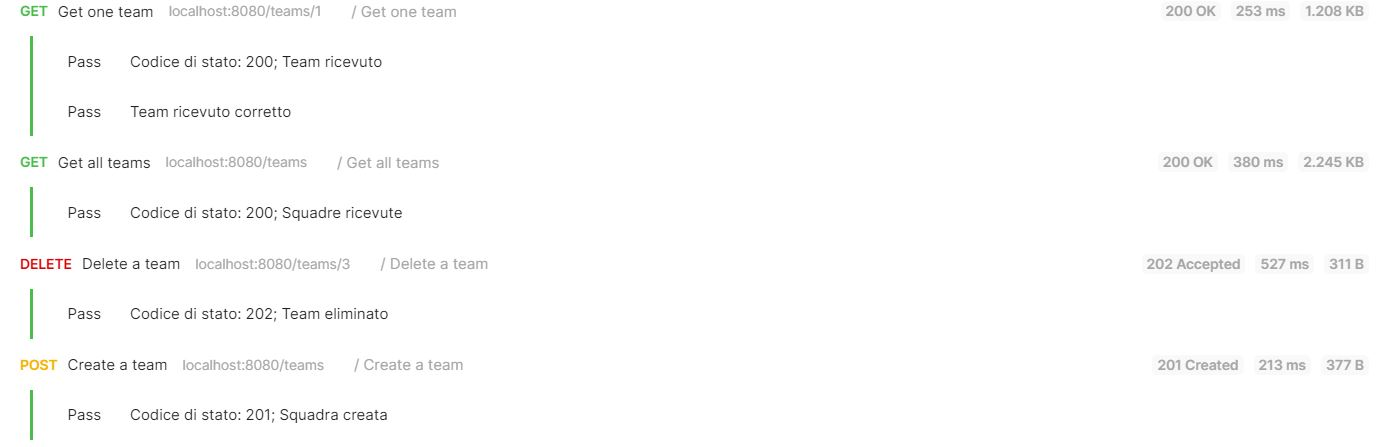
\includegraphics[width=1\linewidth]{./Iterazione 2/ImageFiles/TestTeamController}
		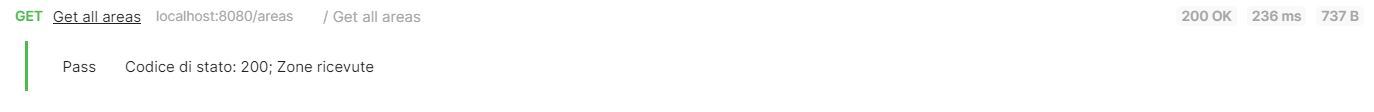
\includegraphics[width=1\linewidth]{./Iterazione 2/ImageFiles/TestAreaController}
		\caption{Risultati test API su Postman.}
		\label{fig:RisultatiTestAPIIT2}
	\end{figure}
\end{itemize}

\clearpage

\subsection{Unit Test}
In questa iterazione è stata testata la funzione \textit{findByUsername()} che permette di recuperare l'utente inserito nel database con lo \textit{username} specificato. Inoltre viene eseguito il test di avvio del framework Spring, inserito di default. Di seguito è riportato il codice del test.

\lstinputlisting[language=Java]{./Iterazione 2/OtherFiles/UserRepositoryTest.java}

Il risultato del test con JUnit ha confermato il corretto funzionamento della funzione.

\begin{figure}[h!]
	\centering
	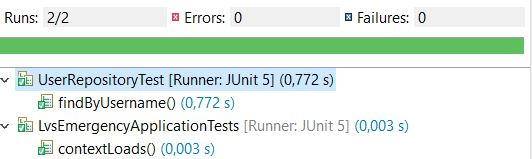
\includegraphics[width=1\linewidth]{./Iterazione 2/ImageFiles/TestJUnit}
	\caption{Risultato test con JUnit.}
	\label{fig:RisultatiTestJunitIT2}
\end{figure}

\subsection{Documentazione API}

\lstinputlisting[language=json]{./Iterazione 2/OtherFiles/getAllAreasResponse.json}

\todo{inserire documentazione API}